% !TEX TS-program = pdflatex
% !TEX encoding = UTF-8 Unicode

% This is a simple template for a LaTeX document using the "article" class.
% See "book", "report", "letter" for other types of document.

\documentclass[11pt]{article} % use larger type; default would be 10pt

\usepackage[utf8]{inputenc} % set input encoding (not needed with XeLaTeX)

%%% Examples of Article customizations
% These packages are optional, depending whether you want the features they provide.
% See the LaTeX Companion or other references for full information.

%%% PAGE DIMENSIONS
\usepackage[top=1.8cm, bottom=1.8cm, left=1.9cm, right=1.9cm]{geometry}
\geometry{a4paper} % or letterpaper (US) or a5paper or....
% \geometry{margins=2in} % for example, change the margins to 2 inches all round
% \geometry{landscape} % set up the page for landscape
%   read geometry.pdf for detailed page layout information

%%% Line Spacing
\usepackage{setspace}
\onehalfspacing

\usepackage{sidecap}

\usepackage{graphicx} % support the \includegraphics command and options

% \usepackage[parfill]{parskip} % Activate to begin paragraphs with an empty line rather than an indent

%%% PACKAGES
\usepackage{booktabs} % for much better looking tables
\usepackage{array} % for better arrays (eg matrices) in maths
\usepackage{verbatim} % adds environment for commenting out blocks of text & for better verbatim
\usepackage{subfig} % make it possible to include more than one captioned figure/table in a single float
\usepackage{amsmath, amssymb, amsthm, lastpage}
% These packages are all incorporated in the memoir class to one degree or another...
\usepackage{url}

%%% HEADERS & FOOTERS
\usepackage{fancyhdr} % This should be set AFTER setting up the page geometry
\pagestyle{fancy} % options: empty , plain , fancy
\renewcommand{\headrulewidth}{0pt} % customise the layout...
\lhead{}\chead{}\rhead{\textit{kwenholz \thepage}}
\lfoot{}\rfoot{}\cfoot{}

%%% SECTION TITLE APPEARANCE
%\usepackage{sectsty}
%\allsectionsfont{\sffamily\mdseries\upshape} % (See the fntguide.pdf for font help)
% (This matches ConTeXt defaults)

%%% ToC (table of contents) APPEARANCE
%\usepackage[nottoc,notlof,notlot]{tocbibind} % Put the bibliography in the ToC
%\usepackage[titles,subfigure]{tocloft} % Alter the style of the Table of Contents
%\renewcommand{\cftsecfont}{\rmfamily\mdseries\upshape}
%\renewcommand{\cftsecpagefont}{\rmfamily\mdseries\upshape} % No bold!

%%% END Article customizations

%%% The "real" document content comes below...
%\date{}

\begin{document}
\begin{titlepage}
    \vspace*{\fill}
    \begin{center}
      \Huge{Where's my Ferry?}\\[0.5cm]
      \Large{Support Vector Machines for Modeling Ferry Tardiness}\\[0.4cm]
      \today
    \end{center}
    \vspace*{\fill}
  \end{titlepage}
\newpage
\vspace*{\fill}
\tableofcontents
\vspace*{\fill}
\newpage

\section{Introduction}
\label{sec:intro}
Ferries (as in \textbf{Figure~\ref{fig:basicferry}} present an interesting 
opportunity to examine a complex traffic system filled with data and affecting 
the lives of many individuals. This paper will discuss a new approach to predicting 
the timeliness of ferries using a support vector machine.  An overview of how 
support vector machines work and their complications in real world use will 
introduce the discussion of how this powerful construct presents a powerful and 
intuitive model for tackling the massive data associated with ferries.  A 
functioning model is developed to examine the complexities of this
approach, the practicality, and as a means of exploring some of the data. 
Additionally, the hypothesis that the addition of weather information improves 
accuracy of the model is explored.

\begin{figure}[h]
  \centering
  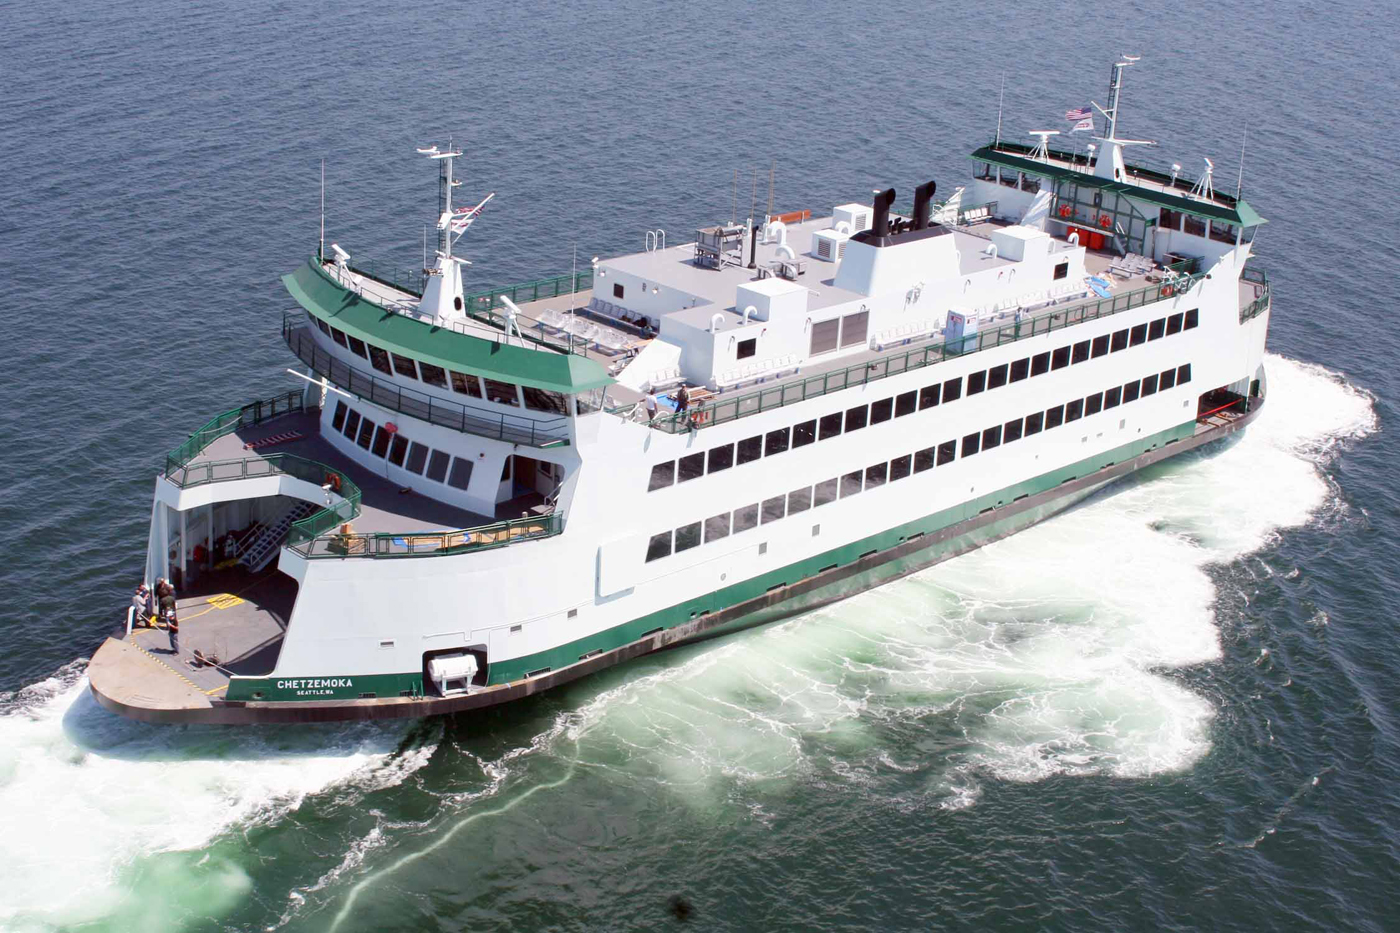
\includegraphics[scale=.15]{images/ferry.jpg}
  \caption{A prototypical WSDOT ferry on its route.}
  \label{fig:basicferry}
\end{figure}

We will attempt to predict the tardiness of ferries, where tardy is 
defined as no less than three minutes later than the
initial (at day's beginning) scheduled arrival or departure time. This definition
of tardiness was chosen to allow for a non-trivial number of tardy events 
(more than 10\% in the data) and to remain practical: i.e. someone could use the
restroom in three minutes time or otherwise make use of that information. The 
Washington State Department of Transportation's ferry system in the Pacific
Northwest served as the source for all data. As will be discussed later on, 
this ferry system is notoriously on time with over 95\% of trips being on 
schedule (within one minute) \cite{wsdotComparison}. This system is of 
particular interest for its sheer volume of passengers: 22 million per year 
\cite{wsfTraffic}.  The volume lends itself well to this project's goals of 
using data mining. 
% TODO: better transition sentence is needed



\section{Preliminaries}
\label{sec:prelims}
Since the goal of the project was to use a large data set for machine learning 
and to develop a model for possibly predict future ferry tardiness, two approaches
popular in available implementations and the literature were initially evaluated:
artificial neural networks (ANNs) and support vector machines (SVMs). These two 
approaches fit into the
category of \textbf{supervised learning}: labeled (known) data is fed into an
algorithm that learns to make better predictions through comparing its own 
predictions to the labeled data set. ANN and SVM are often considered to be
very similar in the problems they attempt to tackle, especially since each can
be used as a linear classifier: a function taking in some object and determining 
a class to which it belongs. Rather than considering tardiness as a spectrum of
degrees, we approach tardiness as a binary feature: late or not. This conceptually
simplifies our problem.  
% TODO: Give examples of how these two are used: spam/ham, cancer, facial recog
If artificial neural networks and support vector 
machines can both solve classification problems, however, which are we supposed
to choose?

\subsection{ANN and SVM}
\label{sec:ann_svm}
Byvatov et al examine the differences of the two approaches for classifying drugs
\cite{byvatov2003comparison}. While their model certainly isn't for a ferry 
system, their discussion suggests data sets with many features (an aspect of the 
ferry model we discuss later) are better suited for SVM, and they also find little
difference in the predictions of ANN and SVM. Most importantly, their conclusion,
and that of their references, is the two approaches are complementary. Each 
tool catches different cases, but the results are comparable in each approach,
and SVM may even require less ``tweaking''. They concede that SVMs are generally
easier to conceptualize, lending a sense of confidence to the work.

Support vector machines are more intuitively motivated. Consider mapping the
features of a ferry trip (time of departure, weather, boat name, etc.) into a
coordinate plane.  Now, if we do this for all the points in our training set,
we can also attach labels to the points (late or not, as in 
\textbf{Figure~\ref{fig:basic_svm_data}}). In two dimensions, we
could try drawing a line through the late and not-late points to separate them.
This line is simply a hyperplane in higher dimensions, and SVM has its theoretical
underpinnings based on the idea of drawing this hyperplane optimally. Apart from
the possible ease of use and understanding, there are also examples of SVM 
being used in similar traffic prediction systems, providing a baseline comparison
and the final reason for choosing SVM over artificial neural networks.

\begin{figure}[h]
  \centering
  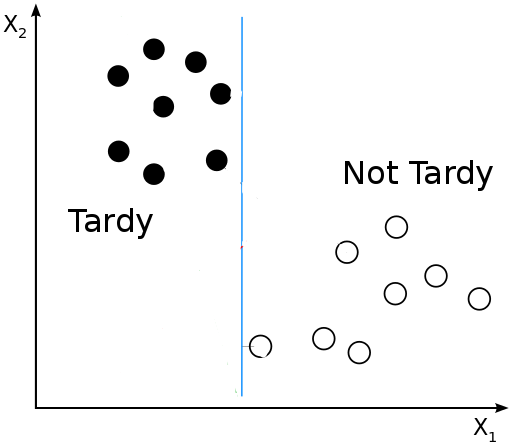
\includegraphics[scale=.5]{images/basic_svm_data.png}
  \caption{A simple example of a separating line for tardiness (i.e. hyperplane). 
      Each data point (or instance) has features $X_1$ and $X_2$.}
  \label{fig:basic_svm_data}
\end{figure}

Smith et al uses SVM to predict the timeliness of airline
traffic in conjunction with weather patterns \cite{smith2008decision}. Their goal is 
to predict the likelihood of requiring a ``ground delay program'': shuffling traffic 
to account for tardiness in the schedule. The model they use involves traffic 
flow management programs to estimate the effects of capacity on an air traffic 
system, and the SVM is trained on labeled data to produce a function predicting 
the need of a ground delay program and/or an actual delay. Their system was
found to be $78\%$ accurate in predicting need of a ground delay program and $83\%$ 
accurate in predicting a delay. Air traffic is much like the ferry system given
its sensitivity to weather, attempt to adhere to a strict schedule, and heavy use.
Due to these similarities, Smith's access to resources like the AMPL supercomputer, 
and his group's expert knowledge, we use $80\%$ as the target accuracy in for the
ferry model. 

It is also noteworthy that SVMs can be used for regression analysis in large
data sets with many variables \cite{chang2011libsvm}. While this paper will not
cover this use of SVM, the possibility of performing such an analysis with the
same tool was one reason in choosing support vector machines.


\subsection{Basics of SVM}
\label{sec:basics_svm}
% FIXME: lame intro sentence
A brief overview of the principles behind support vector machines and their use
will help to lay a basis for the process of the project. As stated earlier,
SVMs are used to find a linear classifier (some function) for a set of data.  In
this project, we seek a way to separate ferry trips that will be three minutes
past their scheduled time (late) or less (on time). To find the linear classifier,
an SVM uses a feature vector, $F$, to describe the trip.  An example $F$ may have
entries for

\[F=\begin{bmatrix}
        EstimatedArrival \\
        BoatName\\
        Temperature\\
        WindSpeed
\end{bmatrix}.\]

This feature vector needs to be entirely numerical, so categorical variables like
boat name must be encoded as numbers.  It is possible to assign boat names to
different values, but most often, it is best to expand the feature like a bit
vector.  If there were boat names \textit{SS Minnow, Death Star,} and 
\textit{Millennium Falcon}, then we would have

\[F=\begin{bmatrix}
        EstimatedArrival \\
        SS\_Minnow\\
        Death\_Star\\
        Millennium\_Falcon\\
        Temperature\\
        WindSpeed
\end{bmatrix}\]

where the entries for boat names are a $1$ if this trip has that name and $0$
otherwise. For reasons detailed in \cite{chang2011libsvm} this is considered 
best practice.

Along with feature vectors for every trip, an SVM uses a weight vector, $w$,
that it is the backbone for the linear classifier. Thus, this $w$ is what the
SVM trains. To determine which class a feature vector corresponds to the
dot product of $F$ and $w$ is taken, with negative values corresponding to 
late and positive values to on time. While training on the labeled data, however,
the SVM adjusts $w$ whenever it predicts incorrectly.  The amount to adjust
can vary based on the implementation, but over time $w$ improves on its ability
to predict the class of any instance in the training set.

An optimal solution to $w$ would form a hyperplane separating the instances
perfectly by class. In \textbf{Figure~\ref{fig:training_hyperplanes}} is an 
example of how an SVM might train a weight vector (represented graphically as
a line) over a set of training data. The final vector, $H_3$, is considered 
optimal because it maximizes the distance between itself and the nearest points
of each class. In the example, it is possible to separate the data with a 
line, but in the real world, and our ferry problem, this is rarely the case.

\begin{figure}[h]
  \centering
  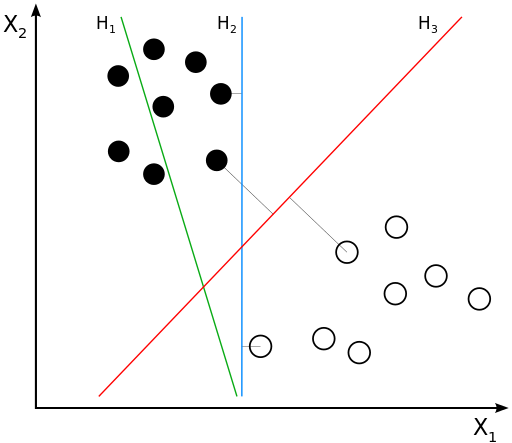
\includegraphics[scale=.5]{images/Svm_separating_hyperplanes.png}
  \caption{As in \textbf{Figure~\ref{fig:basic_svm_data}}, we are trying to separate
    labeled points with a line. An SVM does this iteratively, meaning line $H_1$
    would be the first pass, $H_2$ the result of refitting, and $H_3$ the final 
    classifier produced by the SVM.}
  \label{fig:training_hyperplanes}
\end{figure}

\subsection{Kernel mapping}
\label{sec:kernels}
In \textbf{Figure~\ref{fig:kernel-machine}} is an example of data we can't separate.
Most real world data is like this: inseparable by a hyperplane. The problem this
creates is that we're no longer looking for a linear classifier. A nonlinear 
classifier is required, a significantly more difficult problem. Since no optimal
hyperplane exists, it is difficult to formulate how long an SVM ``look'' for the
hyperplane. We might consider looking for something within reasonable bounds, but 
the kernel trick does away with this problem and brings us back to looking for
a linear classifier \cite{aizerman1964theoretical}.

\begin{figure}[h]
  \centering
  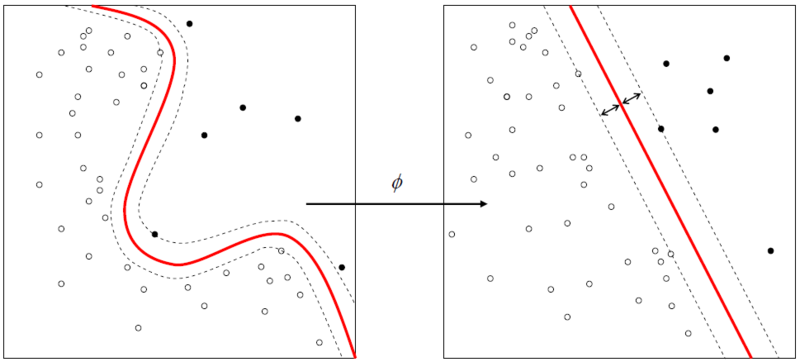
\includegraphics[scale=.6]{images/kernel-machine.png}
  \caption{Separating the data in the first part requires a mapping into a higher
      (often much) dimension. This mapping makes it possible for a learning 
  algorithm like SVM to find at least some separating hyperplane.}
  \label{fig:kernel-machine}
\end{figure}

The kernel trick maps the instances of data into a higher dimensional space 
(often much higher), and the SVM works to find a separating plane in the new 
space. The example in \textbf{Figure~\ref{fig:kernel-machine}} gives an idea
of what the mapping would do to the data. The kernel function used in this 
project is a Gaussian radial basis function and was chosen for its popularity
and since it is built into the LibSVM library \cite{chang2011libsvm} (discussed in
the next section). 

Using the kernel trick requires a small addition to the training process. Optimal
parameters for the kernel function need to be found before fitting with the SVM.
This is done by an exhaustive grid search:
\begin{enumerate}
    \item The user supplies a space of parameters to try.
    \item Within this space, a search grid is created.
    \item Each grid square is ``tried'' by using parameters within to transform
        the data and then run the SVM on a subset of the training data.
\end{enumerate}

So, training the kernel parameters requires training the SVM on very small sets
of data many times to find the best parameters in a space provided by the user.

Implementing all of the functionality of a SVM and kernel function would require
expert knowledge and a thorough amount of validation. Fortunately, libraries to 
work with SVMs and kernel functions already exist.

\subsection{LibSVM}
\label{sec:libsvm}
LibSVM \cite{chang2011libsvm} from Chih-Chung Chang and Chih-Jen Lin provides the
SVM implementation used.  This library has bindings to many languages, is reasonably
straightforward to use from the command-line, is well tested, and has an acceptable
amount of documentation. Using this implementation of an SVM allowed a great deal
of time to be saved and provided a higher degree of certainty in the results.
% TODO: this is weak

\section{Predicting tardiness through data}
\label{sec:problem}
Support vector machines require two sets of labeled data to find a linear classifier:
training and testing. The training data is fed into the SVM as a means of training
the weight vector and finding a linear classifier, and the testing data is used
after this process to check the accuracy of the SVM's product. It is crucial that
these two sets be disjoint. Otherwise, the SVM is basically cheating by being
tested on data it already learned from. There is no clear indicator for how much data
is needed to successfully train an SVM, but too little means the SVM can't 
generalize and too much can cause overfitting. Overfitting is where an SVM is
trained on too much data of similar qualities so that it fails to accurately
classify data of different qualities. This roughly corresponds to finding patterns
which only apply to a small subset of the real instances.  So, it often comes
down to the engineer to determine the appropriate amounts of data for the training
and testing sets based on experience, experimentation, and availability.



\subsection{Washington State's ferries}
\label{sec:wsdot}
The Washington State Department of Transportation (WSDOT) runs the ferry system
in the Pacific Northwest (since 1951) over a stretch of more than 130 miles, from 
Victoria, British Columbia to Point Defiance in Tacoma \cite{wsdotFleet}. The system 
serves over 22 million passengers per year in about $160,000$ sailings 
\cite{wsfTraffic}.  We will refer to one sailing (from one terminal to another) as a 
trip.  \textbf{Figure~\ref{fig:ferry_system}} gives the map of the WSDOT's 20 
terminals and 10 routes, lending perspective to the size of the entire system.

\begin{SCfigure}
  \centering
  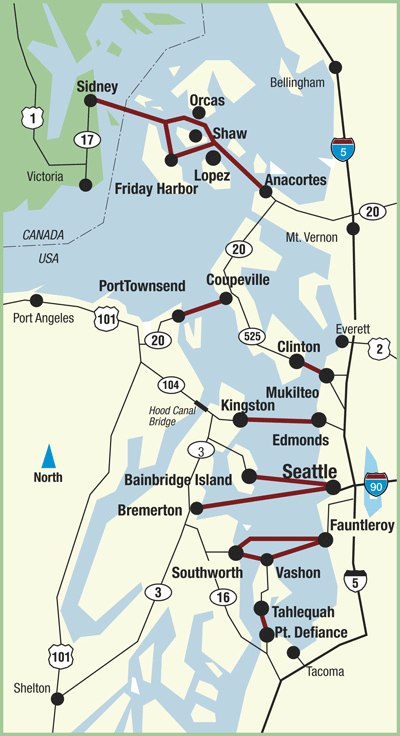
\includegraphics[scale=.4]{images/route-map-overview.png}
  \caption{The Washington State Department of Transportation ferry system. 20
  terminals, making 10 routes, serve users from Point Defiance in Tacoma up to
  Victoria in British Columbia \cite{wsdotVesselWatch}.}
  \label{fig:ferry_system}
\end{SCfigure}

The system is interesting for more than just its traffic. Several of the routes
are rather windy looking, suggesting they may be more susceptible to weather and
traffic delays. Some terminals, furthermore, are a hub for several routes. We
might conjecture these terminals to be susceptible to pileups in traffic. These 
and other complexities of the system make it worthwhile in pursuing the robust 
model provided by an SVM. Fortunately, the complexities and heavy use of the
system seem to have convinced the WSDOT to keep thorough records of the traffic.

To effectively use an SVM, we need enough data we can experiment with and it needs
to be in a uniform, accurate state. Originally, a web scraper was written to grab
information from the WSDOT VesselWatch \cite{wsdotVesselWatch} page, but this was 
made obsolete when a request for information was eventually fulfilled. The WSDOT 
provided, upon request, a record of
approximately $340,000$ ferry trips from October of 2010 to October of 2012. The
data came as a comma separated value file with the nine fields. An example is shown
in \textbf{Figure~\ref{fig:example_wsdot_data}}.

\begin{figure}
    \centering
    \begin{tabular}[h]{lllll}
        \hline
        Vessel & Departing & Arriving & Sched Depart & Actual Depart \\
        \hline
        Kittitas & Mukilteo & Clinton & 9/1/2010 0:00 & 9/1/2010 0:01 \\
        Sealth & Vashon & Southworth & 9/1/2010 0:05 & 9/1/2010 0:06 \\
        Tacoma & Colman & Bainbridge & 9/1/2010 0:15 & 9/1/2010 0:19 \\
    \end{tabular}

    \begin{tabular}[h]{llll}
        \hline
        Initial ETA & Actual Arrival & Date & Route Name\\
        \hline
        9/1/2010 0:13 & 9/1/2010 0:14 & 9/1/2010 & Mukilteo - Clinton \\
        9/1/2010 0:16 & 9/1/2010 0:19 & 9/1/2010 & Southworth - Vashon \\
        9/1/2010 0:45 & 9/1/2010 0:51 & 9/1/2010 & Seattle - Bainbridge Island \\
    \end{tabular}
    \caption{The header of the data provided from the WSDOT (broken into two tables
        to fit page widths). There are over $340,000$ lines in the original file.}
    \label{fig:example_wsdot_data}
\end{figure}

The column headings are all fairly straightforward, but it is worth noting the
scheduled and initial values, for departure and arrival respectively, are the
times found on the schedule for the beginning of the day. With the way the data
is given, we separate out the times into departures and arrivals, creating two
separate scheduling problems. This way it is possible to try predicting arrivals
with the added information of departure time (a seemingly easier problem). 

Before feeding the data into the SVM, it was necessary to transform times and 
categorical variables into numeric values. This was done through several Python
scripts: using seconds past January 1, 1970 for the times and expanding the 
categoricals out as many variables functioning like a bit vector. Additionally,
and a far more difficult problem, we joined this ferry data with weather data
obtained from the National Oceanic and Atmospheric Administration (NOAA).

%       and manage to set the stage for how this research impacts people
%  A portrait of the system</h2>
%       Established in 1951</li>
%        22 million passengers per year</li>
%        20 terminals, 10 routes, 23 vessels</li>
%        Largest ferry system in the world for vehicles</li>
%        From Victoria to Pt. Defiance (~130 miles)</li>
%        159,811 sailings in 2012 (12,764 in December)</li>
%        Almost 10,000,000 vehicles in 2011</li>
%     <img width="110%" 
%      src="images/route-map-overview.gif" align="right">
%  Go over the details of the ferry system.
%  1. history
%  1. Boats
%  2. # Of trips per day
%  3. Routes
%  4. Places serviced
%  6. Design and planning
%  7. Resources for travelers
%    1. Vessel Watch
%    2. Pamphlets
%    3. General knowledge
%    4. Email alerts
%  * Mention that ~95% of boats are on time.  This poses some interesting
%    questions about what we can actually learn.
% 
%  96.4% on time 
%  Best: Pt. Defiance/Tahlequah and Edmonds/Kingston (99.5%)
%  Worst: Anacortes/San Juans (88.9%)
% 

\subsection{Weather and final SVM format}
\label{sec:data_origins}
Retrieving accurate and full historical weather data presented an unexpected 
challenge. Most weather sites are focused on future weather and make historical
data available only through programming APIs which may require a paid subscription.
Fortunately, NOAA provides (by subscription) a portal for retrieving weather data
by station. Stations record over $20$ different features at some point every hour.
It seems that some stations experience outages or are unable to record on some
instruments every so often; because of this, we used the station with the seemingly
most complete data set in the area. This turned out to be a station near the 
Tacoma Narrows Bridge. The data was downloaded in files by month for the range of
October 2010 to October 2012 from a quality controlled store on NOAA's 
site \cite{noaaWeather}. Only about $1,000$ of the more than $24,000$ weather 
entries had to be removed for null values in the wind data.  Unfortunately, 
the station is not a central point, but it seemed close enough at the time. 

We avoided using multiple stations to keep the joining of ferry and weather 
data simpler: since all ferries matched with one station, we just found the 
weather recording closest (within at least an hour) of the actual time reported
on the ferry trip. Of the over $340,000$ ferry trips, only about $13,000$ had to 
be removed.  With a data set so large, this only constituted $4\%$, an acceptable
loss in our case. 

% TODO: What weather data was used (show example of formats and such)


%  </br>
%  ## Weather data (1184 &times; 24)
%      94274,20110101,0053,12,CLR, ,10.00, , , ,25, ,-3.9, ,22, ,-5.4, ,
%      16, ,-8.9, , 69, , 0, ,000, , , ,29.69, ,1, ,002, ,30.04, ,AA, , ,
%      ,30.03, 
% 
%  ## Weather variables 
% 
% talk about the many weather variables I got from NOAA.
% 
%  ## Data monsters 
%    * Python for everything
%    * 1,034 weather recordings missing wind data
%    * 13,220 vessel trips removed from lack of weather data (~ 4%)
%    * Stages of formatting
%        - Combine all weather data files from NOAA
%        - Join ferry and weather data
%        - Handle categorical variables
%        - Make it all SVMable
%  1. Discussion of data quality
%    1. Missing values
%    2. Ill formatted values
%    3. Generally consistent (huge amount so a few mistakes is okay)
%  2. Separated into 290,000 for training and 30,000 for testing
%  2. Suite of Python scripts to cut out bad data
%  3. Scripts to join weather and ferry data
%  4. Performance issues encountered
% 

%  ## Goal refresh 
%  * Find order in the mess: Which features matter?
%  * Do something practical: Can we use the model?
%  * Work with big data: Was all of the data necessary/useful?
% 90 accuracy isn't expected!  This would be weird in most cases.
% This is because it can't be perfect, there is a maximum iter 
% threshold, it's optimization, noise is still noise, 
% 
% Mention the 95% accurate fact and how we can basically be correct
% Most of the time by guessing on time.  We want a model to be similarly
% accurate.
% 

\section{Results}
\label{sec:results}
% TODO: Intro to how a first pass happened, better pass happened, and new hypothesis
%       was tested

\subsection{The first pass}
\label{sec:firstpass}
% TODO: why did this suck?
%  ## SVM is easy right?
%  # <p class="fragment roll-in">No. 60%</p>
%  WHY DID I DO BETTER???
%  1. Accuracy comes from test data (disjoint from train data)
%  1. Needing to fit c and gamma parameters to get better curves
%  2. Duration of runs and sheer size of data sets
% 

\subsection{General results}
\label{sec:gen_results}
% TODO: discuss the general results I had on the ``successful'' runs
% TODO: discuss how the great on-timeness of the system may impact results
% TODO: discuss how weather seemed so strange!
%  ## Results: Arrivals
%  *  Full: 87.0%
%  *  No Weather: 88.0%
%  *  No Departure: 60.0%
%  *  No Departure, No Weather: 59.4%
%  Full = Departure estimate and actual,
%  arrival estimate, vessel name, route, all weather
%  1. How do we know it's correct?
%      1. Classification versus regression: I want a "useful" machine
%      2. Test sets vs. training sets
%  2. Review the numbers of the results
%      1. Results before param fitting of c and gamma
%      1. Departures
%          1. Weather
%          2. No weather
%      2. The more interesting: arrivals
%          1. Weather
%          2. No weather
% 
%  ## Results: Departures
%  * Full: 76.3%
%  * No Weather: 75.7%
%  Full = Departure estimate, vessel name, route, all weather
% 
%       <img width="70%" src="images/route-map-overview.gif" align="right">

\subsection{The problem with weather}
\label{sec:weather_prob}
% TODO: discuss how the experiment withe weather was constructed and carried out
% ## How about that weather?
%  Weather/No Weather
% Without information about the departure, the arrival time
%    predictions were strictly less than 68% accuracy.
%  1. Possible issues
%      1. Location of station
%      2. Poor quality of data
%      3. My error
%      4. Ferries really are consistent enough to not need weather
%  2. Running individual routes
%      1. Closest to Tacoma Narrows
%      2. Middleish (randomly selected)
%      3. Geographically furthest


\section{Closing thoughts}
\label{sec:summary}
% TODO: Recap the results and why SVM was used
%  ## In summary
%  * This is a "cute" model.
%  * Hyperplanes are more than an awesome word.
%  * The ferry system is full of data we can mine.
%  * SVM is like a black box.
 
% TODO: Multiclass SVM?

%  1. Making an actual application
%      1. State of Java web frameworks
%      2. Need to scrape or grab user data
%      3. Update SVM
%  2. Are the schedules online adjusted as time goes by
%  3. Mining the data for patterns
 

% TODO: end with where the work can be taken next
%  ## Future(ish) work
%  * Multi-class SVM for "tardiness categories"
%  * Regression analysis
%  * Graphical application


\newpage 

\bibliographystyle{amsplain}
\bibliography{undergraduate-thesis.bib}

\end{document}

